\documentclass[11pt]{article}
\usepackage{preamble}

\newcommand{\IconChart}{[CHART]}
\newcommand{\entrybox}{\framebox[1.2em]{\rule{0pt}{0.95em}}}
\newcommand{\reciprocalblankgrid}{%
\begin{center}
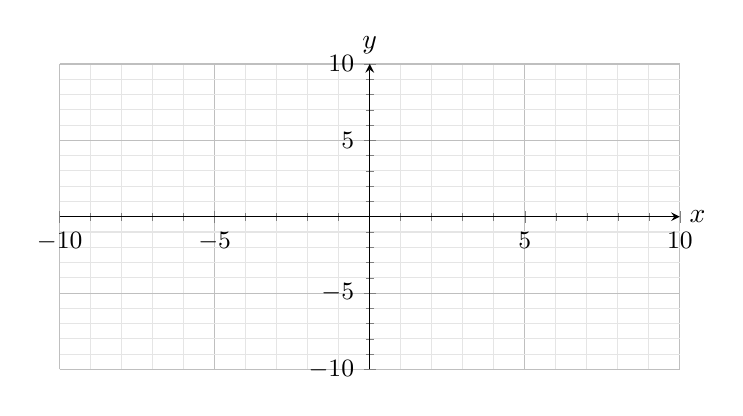
\begin{tikzpicture}
\begin{axis}[
  width=0.78\linewidth,
  height=2.15in,
  xmin=-10, xmax=10,
  ymin=-10, ymax=10,
  axis lines=middle,
  grid=both,
  minor tick num=4,
  xtick={-10,-5,0,5,10},
  ytick={-10,-5,0,5,10},
  tick label style={font=\small},
  label style={font=\small},
  major grid style={draw=black!25},
  minor grid style={draw=black!10},
  xlabel={$x$},
  ylabel={$y$},
  every axis x label/.style={at={(ticklabel* cs:1)},anchor=west},
  every axis y label/.style={at={(ticklabel* cs:1)},anchor=south}
]
\end{axis}
\end{tikzpicture}
\end{center}
}
\newcommand{\gamesblankgrid}{%
\begin{center}
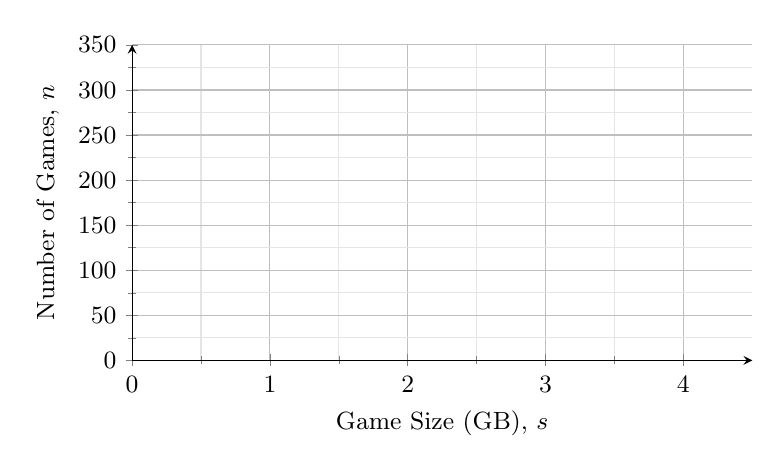
\begin{tikzpicture}
\begin{axis}[
  width=0.78\linewidth,
  height=2.2in,
  xmin=0, xmax=4.5,
  ymin=0, ymax=350,
  axis lines=left,
  grid=both,
  minor tick num=1,
  xtick={0,1,2,3,4},
  ytick={0,50,100,150,200,250,300,350},
  tick label style={font=\small},
  label style={font=\small},
  major grid style={draw=black!25},
  minor grid style={draw=black!10},
  xlabel={Game Size (GB), $s$},
  ylabel={Number of Games, $n$}
]
\end{axis}
\end{tikzpicture}
\end{center}
}
\newcommand{\qelevengraph}{%
\begin{center}
\begin{tikzpicture}
\begin{axis}[
  width=0.74\linewidth,
  height=2.65in,
  xmin=-6, xmax=6,
  ymin=-6, ymax=6,
  axis lines=middle,
  grid=both,
  minor tick num=1,
  xtick={-4,-2,0,2,4},
  ytick={-4,-2,0,2,4},
  tick label style={font=\small},
  label style={font=\small},
  major grid style={draw=black!25},
  minor grid style={draw=black!10},
  clip=false,
  xlabel={$x$},
  ylabel={$y$},
  every axis x label/.style={at={(ticklabel* cs:1)},anchor=west},
  every axis y label/.style={at={(ticklabel* cs:1)},anchor=south}
]
\addplot[warmred, thick, smooth] coordinates {(0.65,6) (1,5) (2,4) (5,1) (5.8,0.7)};
\addplot[warmred, thick, smooth] coordinates {(-5.8,-0.7) (-5,-1) (-2,-4) (-1,-5) (-0.65,-6)};
\addplot[only marks, mark=*, mark size=2.6pt, color=warmred] coordinates {
  (1,5) (2,4) (5,1) (-5,-1) (-2,-4) (-1,-5)
};
\node[text=warmred, anchor=west, font=\small\bfseries] at (axis cs:1.18,5.15) {\((1,5)\)};
\node[text=warmred, anchor=west, font=\small\bfseries] at (axis cs:2.22,4.15) {\((2,4)\)};
\node[text=warmred, anchor=west, font=\small\bfseries] at (axis cs:4.18,1.32) {\((5,1)\)};
\node[text=warmred, anchor=east, font=\small\bfseries] at (axis cs:-4.85,-1.15) {\((-5,-1)\)};
\node[text=warmred, anchor=east, font=\small\bfseries] at (axis cs:-1.78,-3.8) {\((-2,-4)\)};
\node[text=warmred, anchor=east, font=\small\bfseries] at (axis cs:-0.78,-5.1) {\((-1,-5)\)};
\node[text=warmred, font=\Large\bfseries] at (axis cs:4.35,-4.2) {X};
\end{axis}
\end{tikzpicture}
\end{center}
}

\begin{document}

\packetheading{Lesson 4-1 \textperiodcentered\ Period 3 \textperiodcentered\ Student Packet}{Reciprocal Function + Translations --- Assessment-Critical}

\sectionbanner{OBJECTIVES}
{\small
\renewcommand{\arraystretch}{1.25}
\noindent\begin{tabular}{|p{1.8in}|p{4.8in}|}
\hline
\textbf{Math Objective} & Graph the reciprocal function \(f(x) = 1/x\) and its translations \(g(x) = 1/(x-h) + k\). Identify vertical and horizontal asymptotes, state domain and range, and find intercepts where they exist. \\ \hline
\textbf{Language Objective} & Students will use the frame ``This graph is the parent \(f(x) = 1/x\) translated \_\_\_ units \_\_\_. The asymptotes are at \(x =\) \_\_\_ and \(y =\) \_\_\_.'' to describe any translated reciprocal function. \\ \hline
\textbf{Essential Understanding} & The reciprocal function has a vertical asymptote at \(x = 0\) and horizontal asymptote at \(y = 0\). Translations shift the asymptotes: \(g(x) = 1/(x-h) + k\) has asymptotes at \(x = h\) and \(y = k\). The point \((h, k)\) is the new ``center.'' \\ \hline
\end{tabular}
}

\sectionbanner{TOPIC GOALS / ESSENTIAL QUESTION / MATERIALS}
{\small
\renewcommand{\arraystretch}{1.25}
\noindent\begin{tabular}{|p{1.8in}|p{4.8in}|}
\hline
\textbf{Topic Goals} & Students will identify asymptotes and describe translations for 6 reciprocal-function items. This is Topic 4 assessment-prep material. \\ \hline
\textbf{Essential Question} & How do the values of \(h\) and \(k\) in \(g(x) = 1/(x-h) + k\) determine the graph's asymptotes, domain, range, and intercepts? \\ \hline
\textbf{Materials} & Pencils; student packet; graphing calculator (optional, for verification). \\ \hline
\end{tabular}
}

\sectionbanner{LAUNCH --- Reciprocal Function + Translations (teacher models Ex 4 + Ex 5)}

\begin{callout}{\IconBook\ RECIPROCAL FUNCTION --- PARENT \(f(x) = 1/x\)}{calloutgreen}
\textbullet\ Vertical asymptote: \(x = 0\)\\
\textbullet\ Horizontal asymptote: \(y = 0\)\\
\textbullet\ Domain: \(\{x \mid x \neq 0\}\) \hspace{1.8em} \textbullet\ Range: \(\{y \mid y \neq 0\}\)\\
\textbullet\ Graph: hyperbola in Quadrants I and III (two branches, no intersection)
\end{callout}

\begin{callout}{\IconBook\ TRANSLATED RECIPROCAL --- \(g(x) = 1/(x-h) + k\)}{calloutyellow}
\textbullet\ Vertical asymptote shifts to: \(x = h\)\\
\textbullet\ Horizontal asymptote shifts to: \(y = k\)\\
\textbullet\ Domain: \(\{x \mid x \neq h\}\) \hspace{1.8em} \textbullet\ Range: \(\{y \mid y \neq k\}\)\\
\textbullet\ The point \((h, k)\) is the ``new center'' --- where the asymptotes cross.\\
\textbullet\ Example: \(g(x) = 1/(x-3) + 2\) \(\rightarrow\) asymptotes \(x = 3\) and \(y = 2\).

\medskip
To find INTERCEPTS:\\
\hspace*{1.5em}\textbullet\ y-intercept: set \(x = 0\). \(y = 1/(0-h) + k = -1/h + k.\)\\
\hspace*{1.5em}\textbullet\ x-intercept: set \(y = 0\). Solve \(0 = 1/(x-h) + k \rightarrow x = h - 1/k.\)
\end{callout}

\sectionbanner{EXPLORE --- Think-Pair-Share (35 min)}
\textit{Work with a partner. Practice \#19 is assessment-critical (asymptotes + intercepts) --- plan \(\sim\)8 min for it.}

\textbf{Bank-item labels (in order):}
\begin{enumerate}[leftmargin=1.6em,itemsep=2pt,topsep=2pt]
  \item Try It 4 --- Graph \(g(x) = 10/x\) (scaled parent)
  \item Practice \#11 --- Error Analysis: \(y = 5/x\)
  \item Practice \#18 --- Graph \(y = -2/x\) (reflected parent)
  \item Try It 5 --- Graph \(g(x) = 1/(x+2) - 4\) (translated)
  \item Practice \#19 \IconStar\ ASSESSMENT CRITICAL --- \(g(x) = 1/(x-2) + 6\) + intercepts
  \item Practice \#21 --- Video game storage (modeled)
\end{enumerate}

\bankitem{Try It 4 --- Graph \(g(x) = 10/x\) (scaled parent)}{%
Try It 4. Graph the function \(g(x) = 10/x\). What are the domain, range, and asymptotes of the function?
\reciprocalblankgrid
}{}

\bankitem{Practice \#11 --- Error Analysis: \(y = 5/x\)}{%
11. Error Analysis: Describe and correct the error a student made in graphing the function \(y = 5/x\). The student's graph shows labeled points \((1, 5)\), \((2, 4)\), \((5, 1)\) in Quadrant I and \((-5, -1)\), \((-2, -4)\), \((-1, -5)\) in Quadrant III, with a large red X indicating the graph is incorrect.
\qelevengraph
\vspace{0.25in}
}{}

\bankitem{Practice \#18 --- Graph \(y = -2/x\) (reflected parent)}{%
18. Graph the function \(y = -2/x\). What are the domain, range, and asymptotes of the function?
\reciprocalblankgrid
}{}

\bankitem{Try It 5 --- Graph \(g(x) = 1/(x+2) - 4\) (translated)}{%
Try It 5. Graph \(g(x) = 1/(x + 2) - 4\). What are the equations of the asymptotes? What are the domain and range?
\reciprocalblankgrid
}{}

\bankitem{Practice \#19 \IconStar\ ASSESSMENT CRITICAL --- \(g(x) = 1/(x-2) + 6\) + intercepts}{%
19. Graph \(g(x) = 1/(x - 2) + 6\). What are the equations of the asymptotes? What are the domain and range? What are the intercepts?
\reciprocalblankgrid
}{}

\bankitem{Practice \#21 --- Video game storage (modeled)}{%
21. Use Structure: The number of downloaded games that can be stored on a video game system varies inversely with the average size of a video game. A certain video game system can store 160 games when the average size of a game is 2.0 gigabytes (GB).\\

\textbf{(a)} Write an inverse equation that relates the number of games \(n\) that will fit on the video game system as a function of the average game size \(s\) in GB.\\

\textbf{(b)} Use the inverse relationship to complete the table of values.
\begin{center}
\renewcommand{\arraystretch}{1.35}
\begin{tabular}{|l|c|c|c|c|}
\hline
\textbf{Game Size (GB), \(s\)} & 1.0 & 2.5 & 3.0 & 4.0 \\ \hline
\textbf{Number of Games, \(n\)} & \entrybox & \entrybox & \entrybox & \entrybox \\ \hline
\end{tabular}
\end{center}

\textbf{(c)} Sketch a graph of this inverse relationship on a coordinate plane.
\gamesblankgrid
}{}

\sectionbanner{SHARE / SUMMARY (5 min)}

\begin{sentenceframebox}
\textbf{Sentence frames}

Pair share (\#19): ``This graph is the parent \(f(x) = 1/x\) translated \_\_\_ units \_\_\_ and \_\_\_ units \_\_\_. The asymptotes are \(x =\) \_\_\_ and \(y =\) \_\_\_. The intercepts are \_\_\_.''

Whole class: one pair reads \#19. Class signals thumbs up/sideways.
\end{sentenceframebox}

\begin{callout}{\IconChart\ CONCEPT SUMMARY (your reference for Topic 4 assessment)}{calloutell}
INVERSE VARIATION (\(y = k/x\)):\\
\hspace*{1.5em}--- WORDS: As one variable increases, the other decreases; their product \(k\) is constant.\\
\hspace*{1.5em}--- ALGEBRA: \(y = k/x\) where \(k \neq 0\)\\
\hspace*{1.5em}--- GRAPH: parent hyperbola, asymptotes \(x = 0\) and \(y = 0\)

\medskip
RECIPROCAL FUNCTION TRANSLATIONS (\(y = a/(x-h) + k\)):\\
\hspace*{1.5em}--- WORDS: The reciprocal function can shift left/right (\(h\)) and up/down (\(k\)).\\
\hspace*{1.5em}--- ALGEBRA: \(y = a/(x-h) + k\)\\
\hspace*{1.5em}--- GRAPH: asymptotes shift to \(x = h\) and \(y = k\); new ``center'' at \((h, k)\).
\end{callout}

\sectionbanner{EXIT}

\begin{summaryexitbox}{EXIT TICKET --- Pre-Assessment Confidence Check}
I can identify asymptotes of \(y = 1/(x-h) + k\). \hfill Confidence: 1 / 2 / 3 / 4 / 5

I can describe a translation from \(f(x) = 1/x\) to \(g(x)\). \hfill Confidence: 1 / 2 / 3 / 4 / 5

One thing I want to review before Topic 4 assessment: \dotfill
\end{summaryexitbox}

\clearpage

\sectionbanner{OPTIONAL REINFORCEMENT (not collected)}
\textit{Extra stretch for fast finishers. Try without a calculator first.}

\bankitem{Optional \#1  (Savvas SAT/ACT style)}{%
25. SAT/ACT. In a given set of experiments, \(t\) and \(w\) always vary inversely. When \(t = 0.4\) seconds, \(w = 172.8\) grams. How much time has passed when \(w = 14.4\) grams?
}{%
  \answerchoice{A}{2.4 s}
  \answerchoice{B}{4.8 s}
  \answerchoice{C}{27.648 s}
  \answerchoice{D}{995.328 s}
}

\end{document}
